%%%%%%%%%%%%%%%%%%%%%%%%%%%%%%%%%%%%%%%%%%%%%%%%%%%%%%%%%%%%%%%%%%%%%%%%%%%%%%%%
\chapter{Literature Review}\label{ch:literature-review}
%%%%%%%%%%%%%%%%%%%%%%%%%%%%%%%%%%%%%%%%%%%%%%%%%%%%%%%%%%%%%%%%%%%%%%%%%%%%%%%%

%%%%%%%%%%%%%%%%%%%%%%%%%%%%%%%%%%%%%%%%%%%%%%%%%%%%%%%%%%%%%%%%%%%%%%%%%%%%%%%%
\section{A Brief Survey on Traffic Generators}\label{sec:traffic-gen}

A traffic generator is a tool capable of creating and injecting packets into a computer network in a controlled way to generate a synthetic traffic \cite{validate-trafficgen}.  There is a vast variety of traffic generators described on the literature \cite{validate-trafficgen} \cite{ditg-paper} and available in the open-source community\footnote{\href{http://www.icir.org/models/trafficgenerators.html}{http://www.icir.org/models/trafficgenerators.html}}. This is a consequence of an equally large amount of approaches for crafting synthetic traffic \cite{validate-trafficgen}.

The development of new network generators tightly related with to the current needs of network environment, applications sets, and purpose of use \cite{validate-trafficgen}. For example, if we want to evaluate the performance limits of equipment or new technology, you may want to execute stress tests, at specific constant rates. In this case, maximum throughput traffic generator is more interesting. On the other hand, to test how it performs on an actual network environment, you should search for a tool that produces a stochastically realist profile. Or, if you have a more specific usage case, you may search for a traffic generator that emulates an application scenario such as a client and a network server\cite{surge-paper}. 


Alongside with the variety of traffic generators, there are many APIs to create traffic. Some are low-level APIs which enables direct packet injection, such as \textit{libpcap}\cite{web-tcpdump}, \textit{libtins}\cite{web-libtins}, DPDK\cite{web-dpdk} and the GNU C socket library\cite{web-socket}. And there are high-level APIs, provided by traffic generator tools, such as D-ITG\cite{ditg-paper}, Ostinato\cite{web-ostinato} and MoonGen\cite{moongen-paper}. In this case, they enable an easy custom traffic generation and statistics. Also, there are implementations of hardware-based traffic generators using NetFPGAs\footnote{\href{http://netfpga.org/site/\#/}{http://netfpga.org/site/\#/}}.


There are many classifications of traffic generators\cite{sourcesonoff-paper}\cite{hybrid-traffic-gen}\cite{validate-trafficgen}\cite{do-you-trust}, and many have features that fall into more than one class. But classify them it is an efficient way to distinguish the difference between these tools. We will cite here two:

\begin{itemize}
	\item According to its abstraction level \cite{do-you-trust};
	%\item According to its purpose (engine replay, throughput, realism) \cite{validate-trafficgen}
	\item According to its implementation.
\end{itemize}

The most common traffic generator classification in the literature is about its abstraction level\cite{do-you-trust}. There are four groups: Application-level, flow-level, packet-level and multi-level traffic generators. We present a diagram illustrating its concept in figure ~\ref{fig:layers-workload-tools}.

%%%%%%%%%%%%%%%%%%%%%%%%%%%%%%%%%%%%%%%%%%%%%%%%%%%%%%%%%%%%%%%%%%%%%%%%%%%%%%%%
\subsection{According to its abstraction level}

\textbf{Application-level traffic generators}: they try to emulate the behavior of network applications, simulating real workloads stochastically or responsively \footnote{Responsiveness refers to the property of capacity of response over time of the workload tool. That means the behavior of the output may change according to what packets have arrived in the network interface}. As examples, we have Surge\cite{surge-paper}, which emulates the communication between clients and web servers.

\textbf{Flow-level traffic generators}: they are able to configure and reproduce features of flows\cite{do-you-trust}\cite{sourcesonoff-paper}, such as flow duration, start times distributions, and temporal (diurnal) traffic volumes\cite{do-you-trust}. Harpoon \cite{harpoon-paper} is able to extract these parameters from Cisco NetFlow data, collected from  routers.

\textbf{Packet-level traffic generators}: most traffic generators available fall in this class. They can craft and inject packets into the network, and control features like inter-departure times (IDT), packet size(PS), throughput and packets per second\cite{validate-trafficgen}. \cite{validate-trafficgen} classify them as replay engines, maximum throughput generators, and model-based generators. Traffic Replay engines, such TCPreplay\cite{web-tcpreplay}, can read packet capture files (\textit{pcap} files), and inject copies on a network interface. Model-based generators, such D-ITG \cite{ditg-paper}, TG\cite{web-tg}, may have PS and IDT configured by the user. They can configure IDT  either by constant values (defining the packet rate or bandwidth) or by stochastic models. Maximum throughput engines like Ostinato and Seagull are tools that the main goal is to perform end-to-end stress testing. Are included in this category generators that can craft packets from the link layer, like Brute, KUTE, and pktgen.

\textbf{Multi-level traffic generators}: this is a more recent class of network traffic generator. They take into account existing interaction among each layer of the network stack, to create network traffic as close as possible to reality. Today, the most relevant tool is Swing \cite{swing-paper}. Swing take as input collected \textit{pcap} files. Botta at al. \cite{do-you-trust} argues that due its complexity, they are rarely used to conduct experimental researchers. Also, due its complexity, its performance is limited\cite{legotg-paper}. 

% On the other hand, D-ITG reached 9808 Mbps\cite{comparative-trafficgen-tools} in a link of 10 Gbps, but operating as a maximum throughput generator.


\begin{figure}[!ht]
	\centering
	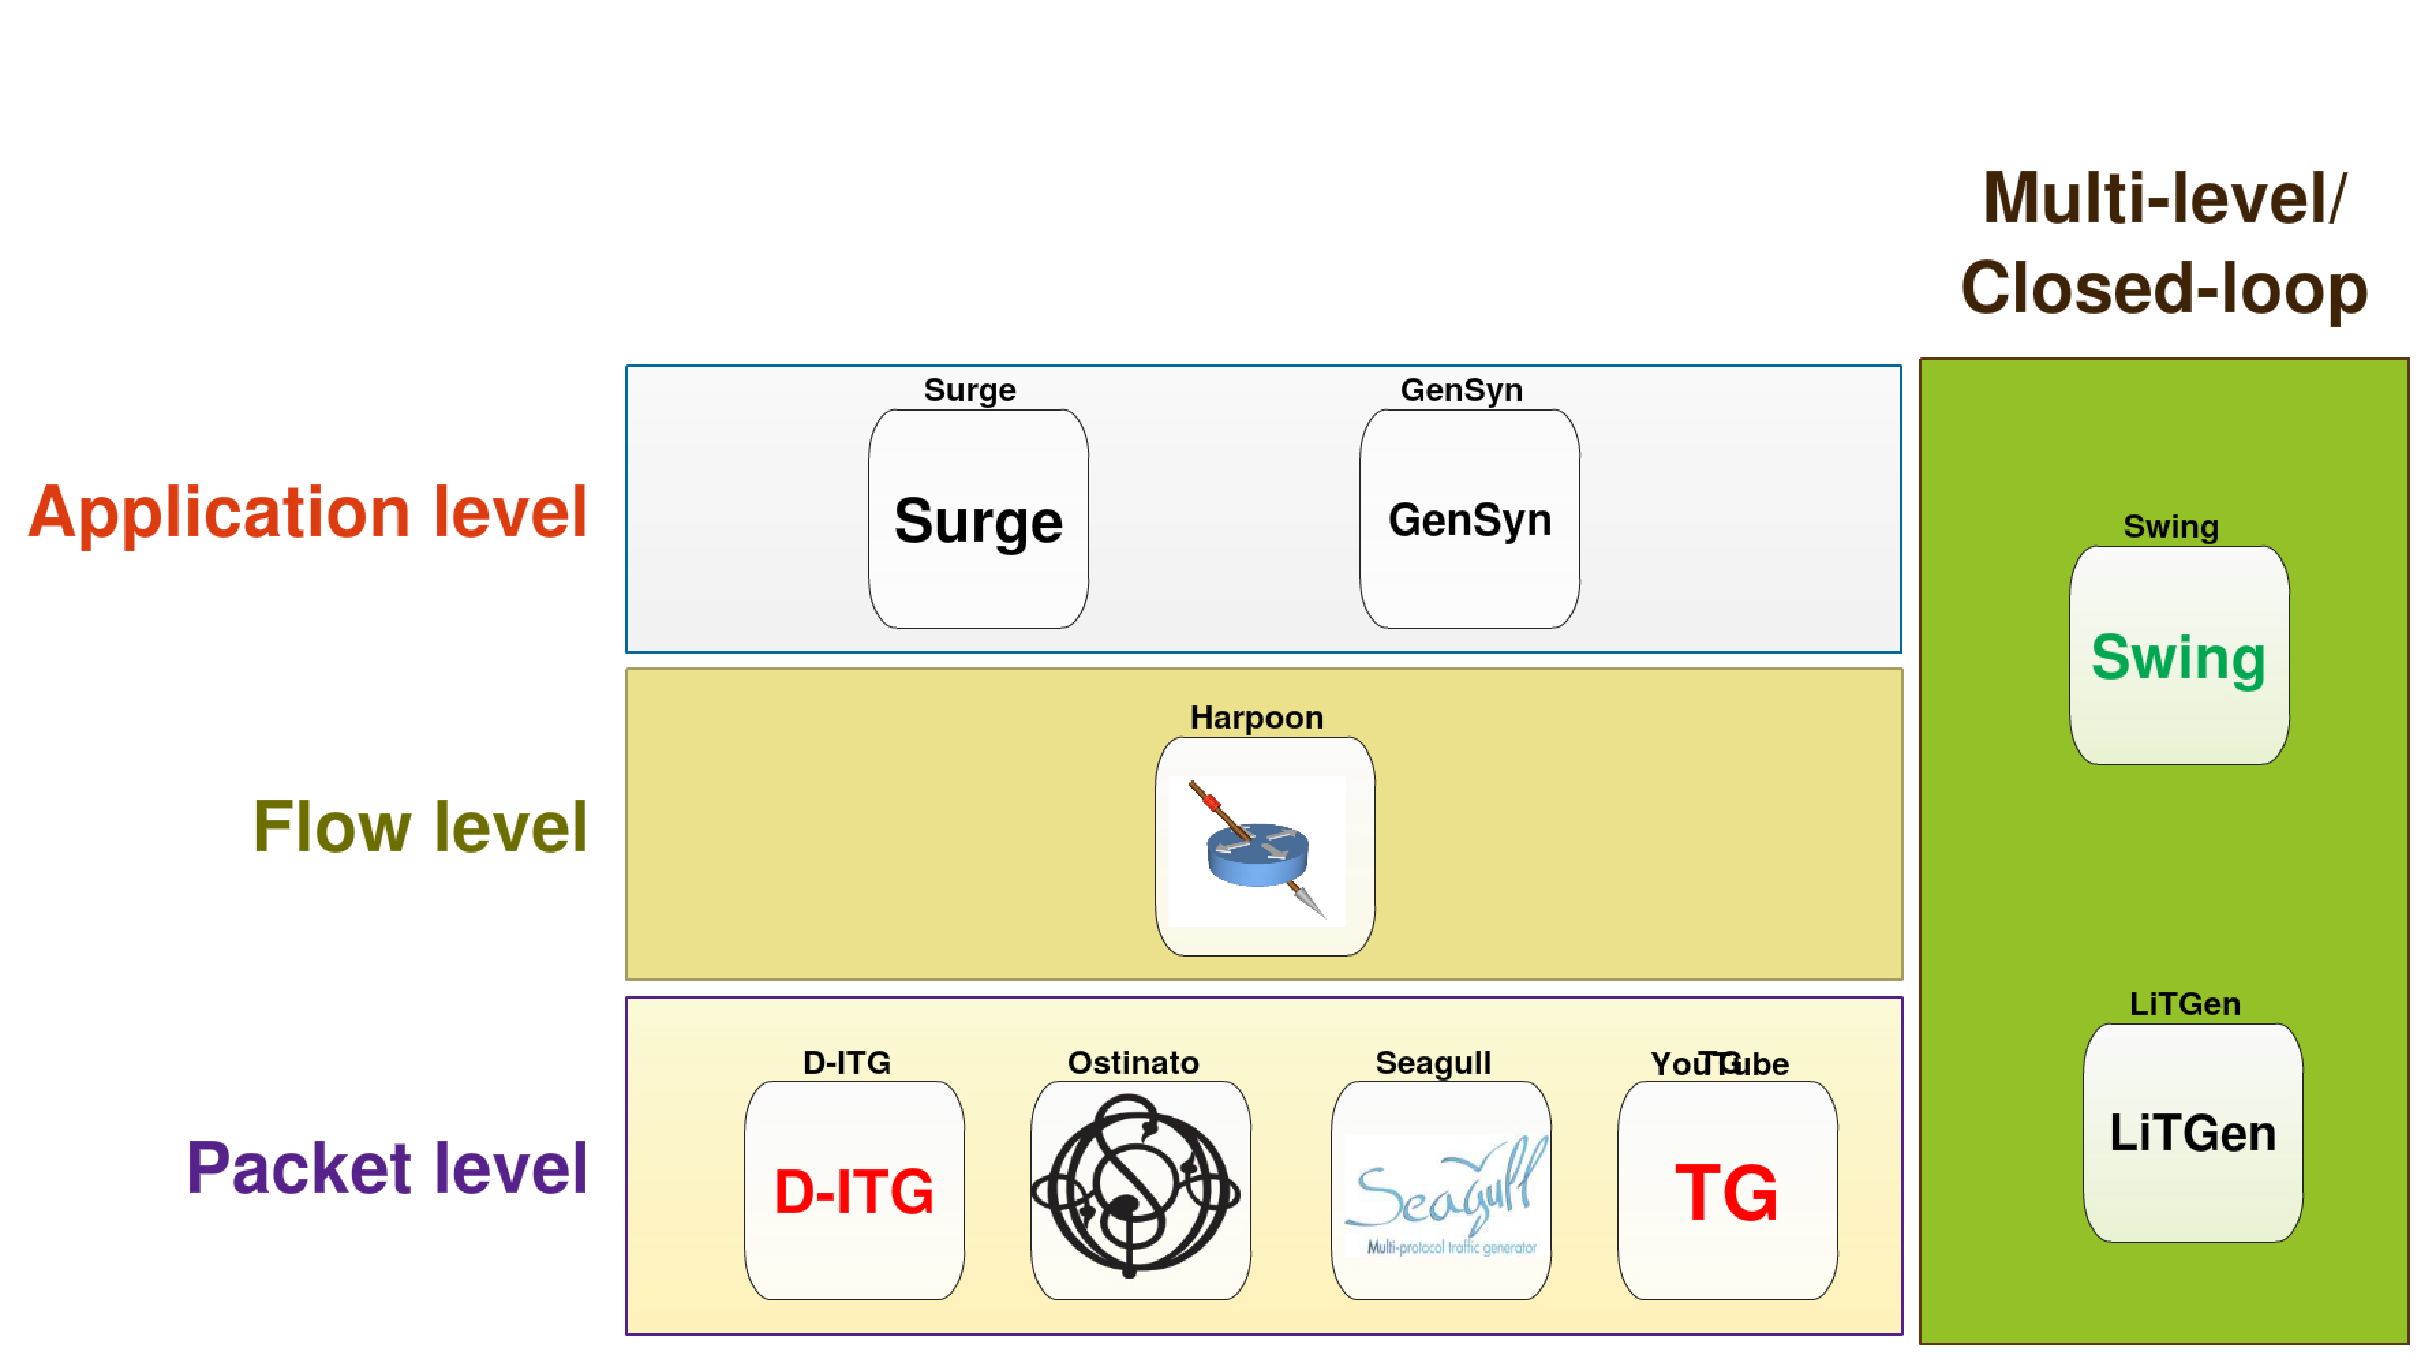
\includegraphics[scale=0.4]{figures/ch2/types-workload-tools}
	\caption{Diagram representing different traffic generators, according to its abstraction layer.}
	\label{fig:layers-workload-tools}
\end{figure}


%%%%%%%%%%%%%%%%%%%%%%%%%%%%%%%%%%%%%%%%%%%%%%%%%%%%%%%%%%%%%%%%%%%%%%%%%%%%%%%%
\subsection{According to its implementation}

\textbf{Software-only traffic generators}: Implementations of traffic generators utterly independent of its running hardware platform. This implementation comprehends most of traffic generator tolls.

\textbf{Software and hardware-dependent traffic generators}: Traffic generators implemented in software, but dependent on the underlying hardware. The most preeminent examples of this class are implemented over DPDK\cite{web-dpdk}. DPDK works directly on the NIC interface, avoiding overheads of the Operational System. As cited on its official website, this approach permits huge precision and speed in the timing of packets, since it can send and receive packets within less than 80 clock cycles.

\textbf{Hardware traffic generators}: This open-source traffic generators implementations are implemented in hardware description language (VHDL/Verilog), and work on NetFPGAs. Some examples of implementations are: PacketGenerator \cite{web-netfpgapacketgenerator}, Caliper \cite{web-caliper}, and OSNT Packet Generator \cite{web-osnt}.


%Tabela: revisao dos principais geradores de trafego
\renewcommand{\tabularxcolumn}[1]{>{\small}m{#1}}


\begin{table}[t!]
\caption{Review of features of some open-source traffic generators}
\begin{center}
\begin{footnotesize}
\begin{tabularx}{\linewidth}{
|>{\hsize=0.9\hsize\raggedright\arraybackslash}X	% 10% of 4\hsize 
|>{\hsize=1.16\hsize\centering\arraybackslash}X					% 30% of 4\hsize
>{\hsize=1.37\hsize\centering\arraybackslash}X					% 30% of 4\hsize
>{\hsize=1.16\hsize\centering\arraybackslash}X					% 30% of 4\hsize
>{\hsize=0.7\hsize\centering\arraybackslash}X					% 30% of 4\hsize
>{\hsize=0.7\hsize\centering\arraybackslash}X|					% 30% of 4\hsize
% sum=4.0\hsize for 4 columns
}
	\hline
	\textbf{Traffic Generator} & 
    \textbf{Operating System} & 
    \textbf{Protocols supported} & 
    \textbf{Stochastic distribution} & 
    \textbf{Interface} & 
    \textbf{Operation Level} \\
    
    \hline
    GenSyn	&
    Java virtual machine &
    TCP, UDP, IPv4 &
    (\textit{user model}, \textit{responsible}) &
    GUI &
    application-level \\
    			
    \hline
    Harpoon &
    FreeBSD 5.1-5.4, Linux 2.2-2.6, MacOS X 10.2-10.4, and Solaris 8-10 &
    TCP, UDP, IPv4, IPv6 &
    (\textit{flow-level model, based on a input trace})&
    CLI &
    flow-level\\    

    \hline
    D-ITG &
    Linux, Windows, Linux Familiar, Montavista, Snapgear &
    IPv4, IPv6, ICMP, TCP, UDP, DCCP, SCTP &
    Constant, uniform, exponential, pareto, cauchy, normal, poisson, gamma, on/off, \textit{pcap}&
    CLI, Script, API &
    packet-level \\
    
    \hline
    Ostinato &
    Linux, Windows, FreeBDS &
    Ethernet/802.3/LLC SNAP; VLAN (with QinQ); ARP, IPv4, IPv6, IP Tunnelling (6over4, 4over6, 4over4, 6over6);TCP, UDP, ICMPv4, ICMPv6, IGMP, MLD; HTTP, SIP, RTSP, NNTP etc... \textit{extensible}&
    constant &
    GUI, CLI, Script, API &
    packet-level\\
	 		
    \hline
    Seagull&
    Linux, Windows &
    IPv4, IPv6, UDP, TCP, SCTP, SSL/TLS and SS7/TCAP. \textit{extensible}&
    constant, poisson, \textit{responsible} &
    CLI, API &
    packet-level\\



    \hline
    PackETH &
    Linux, MacOS, Windows &
    ethernet II, ethernet 802.3, 802.1q, QinQ, ARP, IPv4, IPv6, UDP, TCP, ICMP, ICMPv6, IGMP &
    constant &
    CLI, GUI &
    packet-level \\ 

    \hline
    Iperf &
    Windows, Linux, Android, MacOS X, FreeBSD, OpenBSD, NetBSD, VxWorks, Solaris &
    IPv4, IPv4, UDP, TCP, SCTP &
    constant &
    CLI &
    packet-level \\ 
     
    \hline
\end{tabularx} 
\label{tab:trafficgen-list1}
\end{footnotesize}
\end{center}
\end{table} 
\clearpage

\begin{table}[t!]
\caption{Review of features of some open-source traffic generators}
\begin{center}
\begin{footnotesize}
\begin{tabularx}{\linewidth}{
|>{\hsize=0.9\hsize\raggedright\arraybackslash}X	% 10% of 4\hsize 
|>{\hsize=1.16\hsize\centering\arraybackslash}X					% 30% of 4\hsize
>{\hsize=1.37\hsize\centering\arraybackslash}X					% 30% of 4\hsize
>{\hsize=1.16\hsize\centering\arraybackslash}X					% 30% of 4\hsize
>{\hsize=0.7\hsize\centering\arraybackslash}X					% 30% of 4\hsize
>{\hsize=0.7\hsize\centering\arraybackslash}X|					% 30% of 4\hsize
% sum=4.0\hsize for 4 columns
}
	\hline
	\textbf{Traffic Generator} & 
    \textbf{Operating System} & 
    \textbf{Protocols supported} & 
    \textbf{Stochastic distribution} & 
    \textbf{Interface} & 
    \textbf{Operation Level} \\
   
    \hline
    Swing &
    Linux &
    IPv4, TCP, UDP, HTTP, NAPSTER, NNTP and SMTP &
    \textit{capture trace}  &
    CLI &
    closed-loop and multilevel \\     
   
    \hline
    BRUTE &
    Linux &
    IPv4, IPv6 &
    constant, poisson, trimoda &
    CLI &
    packet-level \\ 
    
         
    \hline
    SourcesOnOff &
    Linux &
    IPv4, TCP, UDP &
    on/off (Weibull, Pareto, Exponential and Gaussian) &
    CLI &
    packet-level \\      
     
     \hline
    TG &
    Linux, FreeBSD, Solaris SunOS &
    IPv4, TCP, UDP &
    Constant, uniform, exponential, on/off &
    CLI &
    packet-level \\ 
    
    \hline
    Mgen &
    Linux(Unix), Windows &
    IPv4, IPv6, UDP, TCP, SINK &
    Constant, exponential, on/off &
    CLI, Script &
    packet-level \\ 

     
     \hline
    KUTE &
    Linux 2.6 &
    UDP &
    constant &
    kernel module &
    packet-level \\ 
     
     \hline
    RUDE \& CRUDE &
    Linux, Solaris SunOS, and FreeBSD &
    IPv4, UDP &
    constant &
    CLI &
    packet-level\\      

     
     \hline
    NetSpec &
    Linux &
    IPv4,UDP, TCP &
    uniform, Normal, log-normal, exponential, Poisson, geometric, Pareto, gamma &
    Script &
    packet-level \\ 
     
     \hline
    Nping &
    Windows, Linux, Mac OS X &
    TCP, UDP, ICMP, IPv4, IPv6, ARP &
    constant &
    CLI &
    packet-level \\ 
     
     
     \hline
    TCPreplay &
    Linux &
    \textit{pcap} &
    constant, \textit{pcap} &
    CLI &
    packet-level (\textit{replay engine}) \\ 

     
     \hline
    TCPivo &
    Linux &
    \textit{pcap} &
    constant, \textit{pcap} &
    CLI &
    packet-level (\textit{replay engine}) \\ 

     \hline
     NetFPGA PacketGenerator &
     Linux &
     \textit{pcap} &
     constant &
     CLI &
     packet-level (\textit{hardware-based}) \\ 

 

    \hline
\end{tabularx} 
\label{tab:trafficgen-list2}
\end{footnotesize}
\end{center}
\end{table} 
\clearpage

\begin{table}[t!]
\caption{Review of features of some open-source traffic generators}
\begin{center}
\begin{footnotesize}
\begin{tabularx}{\linewidth}{
|>{\hsize=0.9\hsize\raggedright\arraybackslash}X	% 10% of 4\hsize 
|>{\hsize=1.16\hsize\centering\arraybackslash}X					% 30% of 4\hsize
>{\hsize=1.37\hsize\centering\arraybackslash}X					% 30% of 4\hsize
>{\hsize=1.16\hsize\centering\arraybackslash}X					% 30% of 4\hsize
>{\hsize=0.7\hsize\centering\arraybackslash}X					% 30% of 4\hsize
>{\hsize=0.7\hsize\centering\arraybackslash}X|					% 30% of 4\hsize
% sum=4.0\hsize for 4 columns
}
	\hline
	\textbf{Traffic Generator} & 
    \textbf{Operating System} & 
    \textbf{Protocols supported} & 
    \textbf{Stochastic distribution} & 
    \textbf{Interface} & 
    \textbf{Operation Level} \\
 
    \hline
    NetFPGA Caliper &
    Linux &
    \textit{pcap} &
    constant &
    CLI &
    packet-level (\textit{hardware-based}) \\  

    \hline
    NetFPGA OSNT &
    Linux &
    \textit{pcap} &
    constant &
    CLI &
    packet-level (\textit{hardware-based}) \\    
 
     \hline
     MoonGen &
     Linux &
     IPv4, IPv6, IPsec, ICMP, UDP, TCP &
     constant, poisson &
     Script API (Lua) &
     packet-level (\textit{hardware-dependent}) \\ 
     
    \hline
    Dpdk Pktgen &
    Linux &
    IPv4, IPv6, ARP, ICMP, TCP, UDP, \textit{pcap} &
    constant, \textit{pcap} &
    CLI, Script API (Lua) &
    packet-level (\textit{hardware-dependent})\\      
     
     \hline
     Dpdk NFPA &
     Linux &
     \textit{pcap} &
     constant, \textit{pcap} &
     CLI, Web &
     packet-level (\textit{hardware-dependent}) \\ 
     
     \hline
     LegoTG &
     Linux &
     \footnote{Depend on underlying tools used} &
     \footnote{Depend on underlying tools used}  &
     CLI, Script &
     packet-level \\  
 
     \hline
     LiTGen &
     \textit{missingInfo} &
     \textit{missingInfo} &
     \textit{wifi model} &
     \textit{missingInfo} &
     closed-loop and multilevel\\   
 
     \hline 
     gen\_send/ gen\_recv &
     Solaris, FreeBSD, AIX4.1, Linux &
     UDP &
     constant &
     CLI &
     packet-level \\

     \hline 
     mxtraf &
     Linux &
     TCP, UDP, IPv4 &
     constant &
     GUI, script &
     packet-level \\

     \hline 
     Jigs Traffic Generator (JTG) &
     Linux &
     TCP, UDP, IPv4, IPv6 &
     constant &
     CLI &
     packet-level \\

     \hline 
     SURGE &
     Linux &
     TCP, IPv4 &
     \textit{application model} &
     CLI &
     application-level\\


     \hline 
     Httperf  &
     Linux &
     TCP, IPv4 &
     \textit{application model} &
     CLI &
     aplication-level \\


     \hline 
     VoIP Traffic Generator &
     Linux &
     UDP, IPv4 &
     \textit{application model} &
     CLI &
     application-level \\

    \hline
\end{tabularx} 
\label{tab:trafficgen-list3}
\end{footnotesize}
\end{center}
\end{table} 
\clearpage




%%%%%%%%%%%%%%%%%%%%%%%%%%%%%%%%%%%%%%%%%%%%%%%%%%%%%%%%%%%%%%%%%%%%%%%%%%%%%%%%
\section{Network Traffic Modeling and Realistic Traffic Generation}\label{sec:modeling-traffic}


Along with the huge diversity of traffic generator tools, there are many traffic generation approaches, depending on the main purpose of the traffic generator. Maximum throughput traffic generators have in mind the idea of sending as much traffic through an interface as it can. But the generation of a realistic workload is a need for validation of many aspects of a new infrastructure. First, to generate a realist traffic, we need to define the complexity that our synthetic traffic must have, compared to real ones. Depending on our purpose, we may focus on one or more aspects of the traffic. For example, protocols, header customization, packet-level features (inter-departure, packet-size) and flow level features (number of flows and flow modeling).


As presented, there is a huge amount of open-source traffic generators available. Each of them with many different sets of features available. But, on the generation of realistic workload, the set of possibilities become much more restrict. On the other hand, there are many works on characterization, modeling, and simulation of different types of network workload \cite{ditg-paper}.


As stated by Botta et al.\cite{ditg-paper},  a synthetic network workload generation over real networks should be able to: (1) Capture real traces complexity over different scenarios; (2) Be able to custom change some specific properties generated traffic ; (3) Return measure indicators of performance experienced by the workload.


To generate realistic traffic workloads, two main approaches exist in the literature \cite{ditg-paper}. First, we have the trace-based generation, where replay engines generate the traffic. As examples, we have TCPreplay, TCPivo, and others. The other approach is an analytical model-based generation. In this case, the packet generation process depends on analytical and stochastic models. As examples of tools, we have Swing, D-ITG, TG, MGEN RUDE/CRUDE, Seagull, and many others.  These tools control traffic features using stochastic and analytical models and/or enable header customization. 


The advantage of the replay engine is its simplicity. There is no need for stochastic modeling of features. It just needs to know how to read the packet from a file, called \textit{pcap}, and replicate it on the internet interface. Most of the traffic features such as packet sizes, inter-departure, and packet headers will be realistic. But, its major issue is the storage space required to generate traffic without replication. In fact, depending on the throughput required, just some seconds of traffic replication will cost GB's of hard disk space. If it is necessary to generate traffic for a longer time, or good \textit{pcaps} traces are not available, analytical are necessary. 


Classical models for network traffic generation were the same used in telephone traffic, such as pure Poisson or Poisson-related, like Markov and Poisson-batch\cite{selfsimilar-ethernet}. They are able to describe the randomness of an Ethernet link but cannot capture the presence of "burstiness" in a long-term time scale, such as traffic "spikes" on long-range "ripples" \cite{selfsimilar-ethernet}. In fact, as we can see at \cite{selfsimilar-ethernet} the nature of the Ethernet traffic is self-similar. It has a fractal-like shape since characteristics seen in a small time scale should appear on a long-scale as well. This is most of the time referred as long-range dependence or degree of long-range dependence (LRD). One way to identify if a process is self-similar is checking its Hurst parameter, or Hurst exponent H, as a measure of the "burstiness" and LRD. In fact, a random process is self-similar and LRD  if 0.5 < H < 1 \cite{stochartic-selfsimilar}. Furthermore, some later studies advocate the use of more advanced multiscaling models (multifractal), addressed by investigations that state multifractal characteristics.

Another desired characteristic is a high variability, in mathematical terms, an infinite variance. Process with such characteristic is said to be heavy-tailed \cite{sourcesonoff-paper}. In practical terms, that means a sudden discontinuous change can always occur. Heavy tail means that a stochastic distribution is not exponentially bounded\cite{sourcesonoff-paper}. This means that a value far from the mean does not have a negligible probability of occurrence. We can express self-similar and heavy-tailed processes using heavy-tailed stochastic distributions, such as Pareto and Weibull. As a reference for these stochastic distributions, a list in the table ~\ref{tab:distributions-equations}. In the last column, we indicate if the distribution is or not heavy-tailed.

\begin{table}[t!]
\centering
\caption{Probability density function (PDF) and Cumulative distribution function (CDF) of some random variables, and if this stochastic distribution has or not self-similarity property. Some functions used to express these distributions are defined at the table ~\ref{tab:distributions-definitions} }
\label{tab:distributions-equations}
\scalebox{0.82}{ 
\begin{tabular}{lcccr}
Distribution & PDF Equation & CDF Equation & Parameters & Heavy-tailed\\ \hline
\\
\multirow{2}{*}{Poisson} & \multirow{2}{*}{$f[k] = \frac{e^{-\lambda}\lambda^k}{k!}$} & \multirow{2}{*}{$F[k] = \frac{\Gamma(\lfloor k + 1 \rfloor, \lambda)}{ \lfloor k \rfloor!}$} &  $\lambda > 0$  (mean, \\
 &  &  & variance) & no \\ 
\\ 
\multirow{2}{*}{Binomial} & \multirow{2}{*}{$f[k] = \binom{n}{k}p^{k}(1 - p)^{n - k} $} & \multirow{2}{*}{$F[k] = I_{1 - p}(n - k, 1 + k)$} &  $n > 0$ (trials)\\  &  &  &$p > 0$ (success)  & no \\ 
\\
\multirow{2}{*}{Normal} & \multirow{2}{*}{$f(t) =  \frac{1}{\sqrt[]{2\sigma^2}\pi}e^{\frac{(t - \mu)^2}{2\sigma^2}}$ } & \multirow{2}{*}{ $F(t) = \frac{1}{2}[ 1 + \text{erf}(\frac{t - \mu}{\sigma\sqrt[]{2}})]$ } &  $\mu$ (mean) \\ &  &  & $\sigma > 0$ (std.dev) & no \\ 
\\ 
\multirow{2}{*}{Exponential} & \multirow{2}{*}{ $f(t) = \begin{cases} \lambda e^{-\lambda t} ;& t \geq 0 \\ 0;& t < 0 \end{cases} $  }   & \multirow{2}{*}{ $F(t) = 1 - e^{-\lambda t} $ } & \\ &  &  & $\lambda > 0$ (rate)  & no \\ 
\\
\multirow{2}{*}{Pareto} & \multirow{2}{*}{$f(t) = \begin{cases} \frac{\alpha t_{m}^\alpha}{t^{\alpha + 1}} ;& t \geq t_{m} \\ 0;& t < t_{m} \end{cases} $ } & \multirow{2}{*}{$F(t) = \begin{cases} 1 - (\frac{t_{m}}{t})^\alpha ;& t \geq t_{m} \\ 0;& t < t_{m}\end{cases} $} &  $\alpha > 0$ (shape)  \\ & &  &  $t_{m} > 0$ (scale)   & yes \\ 
\\ 
\multirow{2}{*}{Cauchy} & \multirow{2}{*}{ $f(t) = \frac{1}{\pi \gamma}[\frac{\gamma^2}{(t - t_{0})^{2} + \gamma^{2}}]$ } & \multirow{2}{*}{ $F(t) = \frac{1}{\pi}\arctan( \frac{t - t_{0}}{\gamma} ) + \frac{1}{2}  $ } &  $\gamma > 0$ (scale) \\ &  &   & $t_{0} > 0$ (location) & yes \\  
\\
\multirow{2}{*}{Weibull} & \multirow{2}{*}{ $f(t) = \begin{cases} \frac{\alpha}{\beta^\alpha}t^{\alpha - 1}e^{(t/\beta)^{\alpha}}; & t \geq 0 \\ 0; & t < 0 \end{cases}$  } & \multirow{2}{*}{ $F(t) = \begin{cases} 1 - e^{-(t/\beta)^{\alpha}}; & t \geq 0 \\ 0 ; & t < 0  \end{cases}$ } & $\alpha  > 0 $ (shape) \\ &  &  & $\beta > 0$ (scale)  & yes \\
\\
\multirow{2}{*}{Gamma} & \multirow{2}{*}{ $ f(t) = \frac{\beta^{\alpha}}{\Gamma(\alpha)}t^{\alpha - 1}e^{-\beta t}  $ } & \multirow{2}{*}{$ F(t) = 1 - \frac{1}{\Gamma(\alpha)}\Gamma(\alpha, \beta x) $} & $\alpha > 0$ (shape) \\ &  &  & $\beta > 0$ (rate) & no \\
\\ 
%\multirow{2}{*}{Student's t} & \multirow{2}{*}{} & \multirow{2}{*}{} &  \\ &  &  & & \\ 
%\\
\multirow{2}{*}{Beta} & \multirow{2}{*}{ $ f(t) = \frac{x^{\alpha - 1}(1 - x)^{\beta - 1}}{B(\alpha, \beta)} $ } & \multirow{2}{*}{ $ F(t) = I_{x}(\alpha, \beta) $ } &  $\alpha > 0$ (shape) \\ &  &  & $\beta > 0$ (shape) & no \\ 
\\ 
\multirow{2}{*}{Log-normal} & \multirow{2}{*}{ $ f(t) = \frac{1}{t \sigma \sqrt[]{2 \pi}}e^{- \frac{(\ln(x) - \mu)^{2}}{2 \sigma^{2}}} $ } & \multirow{2}{*}{ $ F(t) = \frac{1}{2} + \frac{1}{2}\text{erf}[\frac{\ln(x) - \mu}{\sqrt[]{2} \sigma}] $ } & $\mu$ (location)\\
 &  &  & $ \sigma > 0 $ (shape) & yes \\ 
\\
\multirow{2}{*}{Chi-squared} & \multirow{2}{*}{ $ f(t) = \frac{1}{2^{\frac{k}{2}}\Gamma(\frac{k}{2}) }t^{\frac{k}{2} - 1}e^{-\frac{t}{2}} $ } & \multirow{2}{*}{ $ F(t) = \frac{1}{\Gamma(\frac{k}{2})}\gamma(\frac{k}{2}, \frac{x}{2}) $ } &  \\
 &  &  & $ k \in \mathbb{N}_{>0} $ &  no\\ 
\\
 
\hline
\end{tabular} 
} %scalebox
\end{table}

\begin{table}[t!]
\centering
\caption{Definitions of some functions used by PDFs and CDFs}
\label{tab:distributions-definitions}
\begin{tabular}{ll}
\hline
Function                             & Definition \\ 
\hline
\\
Regularized Incomplete beta function & $ I_{x}(a, b) = \frac{B(x| a, b)}{B(a, b)} $           \\
\\
Incomplete beta function             & $ B(x| a, b) = \int_{0}^{x} t^{a - 1} (1 - t)^{(b - 1)} \text{d}t $           \\
\\
Beta function                        & $ B(x| a, b) = \int_{0}^{1} t^{a - 1} (1 - t)^{(b - 1)} \text{d}t $           \\
\\
Error function                       & $ \text{erf}(x) = \frac{1}{\sqrt[]{\pi}}\int_{x}^{-x} e^{-t^{2}} \text{d}t $           \\ 
\\
Lower incomplete Gamma function      & $ \gamma(s, x) = x^{s}\Gamma(s)e^{-x}\sum_{k = 0}^{\infty}\frac{x^{k}}{\Gamma(s+k+1)} $  \\
\\
\hline
\end{tabular}
\end{table}


We call these concepts of High variability and Self-similarity Noah and Joseph Effects \cite{selfsimilar-highvariability}. We can see at\cite{selfsimilar-highvariability} that a superposition of many ON/OFF sources (or packet trains) using ON and OFF that obey the Noah Effect (heavy-tailed probabilistic functions), also obey the Joseph effect. That means, it is self-similar and we can use to describe an Ethernet traffic. As we can see, some works on the literature on synthetic traffic uses this principle, like sourcesOnOff\cite{sourcesonoff-paper}, or have to support models like D-ITG\cite{ditg-paper}.


An accurate replication of a workload should be able to control packet headers such as QoS fields, protocols, ports, addresses, and so on. Traffic generators provide support for these features, more frequently in a limitted way. Most offer support just common protocols, such as TCP, UDP, and IPv4. On the other hands, there are some which provide a huge variety of support and control over packet headers like PackETH\cite{web-packeth} and D-ITG. Other tools are even able to enable you to extend this feature and develop support to new protocols. For example, Ostinato and Seagull permit you to define your own customized protocol.

%revisão da sessão 0.1 até aqui

An important desirable feature that should be controlled is the packet size distribution since each flow may have its own packet distribution. As we can see in many works, the packet size of a trace may result in a huge impact in a trace throughput \cite{stochartic-selfsimilar}\cite{performance-trafficgen}; small packets cause a huge overhead in the packet throughput. In the table ~\ref{tab:packet-size-impact} there are a survey of results found by two different works \cite{comparative-trafficgen-tools} \cite{performance-trafficgen} about the impact of different packet sizes in the throughput rate.Therefore, it is an important factor we must taken into account in the evaluation of new proposals, and in the implementation of network workloads generators. On packet size distribution characterization, we can find many works in the literature. For example, \cite{packet-distribution-model} analyses many packet sizes distributions of many packet traces, in many environments. Some general results are that 90\% of UDP packets are smaller than 500 bytes, and most packets transmitted using TCP have 40 bytes (acknowledgment) and 1500 bytes (Maximum Transmission Unit, MTU) \cite{packet-distribution-model}. For UDP traffic, we have similar results, since mostly they are bimodal as well \cite{udp-flows-model}. Ostrowsky et al.\cite{udp-flows-model} found that, on UDP traces the modes of two regions are 120 and 1350 bytes, with a cut-off value of 750 bytes. They also find that roughly UDP packets constitute 20\% of the total number of packets on captures. 


\begin{table}[t!]
\centering
\caption{Two different studies evaluating the impact of packet size on the throughput. Both compare many available open-source tools on different testbeds. In all cases, small packet sizes penalize the throughput. Bigger packet sizes achieve a higher throughput.}
\label{tab:packet-size-impact}
\scalebox{0.9}{
\begin{tabular}{|l|c|c|c|}
\hline
 & \multicolumn{3}{c|}{Traffic Generators} \\ \cline{2-4} 
\multicolumn{1}{|c|}{Article and setup} &  & \multicolumn{1}{c|}{Maximum bit-rate} & \multicolumn{1}{c|}{Maximum bit-rate} \\
 & \multicolumn{1}{c|}{Toll} & \multicolumn{1}{c|}{\begin{tabular}[c]{@{}c@{}}at small packet \\ sizes\end{tabular}} & \multicolumn{1}{c|}{\begin{tabular}[c]{@{}c@{}}at big packet \\ sizes\end{tabular}} \\ \hline
\textit{\begin{tabular}[c]{@{}l@{}}Comparative study of various \\ Traffic Generator Tools \cite{comparative-trafficgen-tools} ;\end{tabular}} & PackETH & 150 @(64 bytes) & 1745 @(1408 bytes) \\ \cline{2-4} 
\begin{tabular}[c]{@{}l@{}}setup: Linux (Centos 6.2, \\ Kernel version 2.6.32),\end{tabular} & Ostinato & 135 @(64 bytes) & 2850 @(1408 bytes) \\ \cline{2-4} 
\begin{tabular}[c]{@{}l@{}}Inter(R) Xeon(R) CPU with 2.96GHz,\\  RAM of 64GB , NIC Mellanox\end{tabular} & D-ITG & 62 @(64 bytes) & 1950 @(1408 bytes), \\
\begin{tabular}[c]{@{}l@{}}Technologies MT25418 {[}ConnectXVPI \\ PCIe 2.0 2.5GT/s - IB DDR{]}\end{tabular} &  &  & \begin{tabular}[c]{@{}l@{}}9808 @(1460 bytes, \\ 12 threads)\end{tabular} \\ \cline{2-4} 
10 Bbps. Protocol: TCP & Iperf & * & \begin{tabular}[c]{@{}l@{}}8450 @(1460 bytes, \\ 12 threads)\end{tabular} \\ \hline
\textit{\begin{tabular}[c]{@{}l@{}}Performance Monitoring of Various \\ Network Traffic Generators \cite{performance-trafficgen};\end{tabular}} & Iperf & 46.0 @(128 bytes) & 93.1 @(1408 bytes) \\ \cline{2-4} 
\begin{tabular}[c]{@{}l@{}}Inter(R) Pentium 4(R), CPU \\ with 3.0GHz, RAM 1GB,\end{tabular} & Netperf & 46.0 @(128 bytes) & 89.9 @(1408 bytes) \\ \cline{2-4} 
\begin{tabular}[c]{@{}l@{}}NIC Intel Pro/100 Adapter \\ (100Mbps),\end{tabular} & D-ITG & 38.1 @(128 bytes) & 83.1 @(1408 bytes) \\ \cline{2-4} 
\begin{tabular}[c]{@{}l@{}}Hard Drivers Seagate Barracuda \\ 7200 series with 20BG. \\ Protocol:TCP\end{tabular} & IP Traffic & 61.0 @(128 bytes) & 76.7 @(1408 bytes) \\ \hline
\end{tabular}
}
\end{table}


As could be expected, router capture traces, are mostly bimodal, since most of the traffic in backbones is TCP. But, the size of the each mode may change depending on the application. For example, a www usage tends to have a mode close to the MTU higher if compared to an FTP capture. So, for packet workload generation, these results suggest the importance of controlling the packet size behavior for each flow\cite{packet-distribution-model}.

On flow level traffic generation, some packet-level traffic generators permit the control of flow generation, mostly by manually controlling headers parameters through an API or via scripting. In terms of automatic flow configuration, an example is Harpoon\cite{harpoon-paper} which can to automatic configure its flows, using as input NetFlow Cisco traffic traces to automatically setting parameters. Harpoon deals with flow modeling in three different levels: file level, session level, and user level, not dealing with packet level at all.  In the file level, Harpoon model two parameters:  the size of files being transferred, and the time interval between consecutive file requests, called inter-file request time. The middle level is the session level, that consist of sequences files transfer between two distinct IP addresses. The session level has three components: the IP spatial distribution, the second is the inter-session start times and the third is the session duration. The last level is the user level. In Harpoon, "users" are divided on "TCP" and "UDP" users. Which conduct consecutive session using these protocols. This level has two components: the user ON time, and the number of active users. By modeling the number of users, harpoon can reproduce temporal(diurnal) traffic volumes, which is an interesting feature, once it is common on Internet traffic. 

A feature that may be highly desirable for realistic traffic generation is  operating in closed-loop like Swing\cite{swing-paper}. This means when the changes its behavior at run time according to the observation made in real-time, with involves modification of the traffic to be generated \cite{ditg-paper}. These modifications involve changes on parameters of statistical distributions of inter-departure time (IDT) and packet size (PS).

Closed-loop multi-layer and application layer traffic generators also models application and user behavior, like the number of request/response exchanges per connection, response sizes, request sizes, user think time between connections, the number of RREs, RREs think time, etc \cite{swing-paper}.

Finally, on newly arrived internet scenarios, due its increasing complexity of networks and the rise of many new technologies, such as SDN\cite{sdn-survey} and NFV\cite{nfv-challenges}; which include the replacement of old and reliable technologies by new and not as strongly validated ones. In this sense that a point to point validation is not enough anymore, an arriving requirement is the distributed workload generator, which includes a logically centralized module such as a controller\cite{ditg-paper}, or an orchestrator\cite{legotg-paper}, able to control and synchronize and deploy workloads of many different hots. As examples, D-ITG API gives this possibility via daemons, and LegoTG\cite{legotg-paper} Framework implements a complete and easily extensible orchestrator. Due new scenarios where virtualization network functions and hardware is overcoming hardware, a logically centralized control and orchestration of synthetic workloads is a feature that easy the work\cite{legotg-paper}.


%%%%%%%%%%%%%%%%%%%%%%%%%%%%%%%%%%%%%%%%%%%%%%%%%%%%%%%%%%%%%%%%%%%%%%%%%%%%%%%%
\section{Validation of Traffic Generator Tools}~\label{sec:validation-traffic-gen}

After the implementation of a traffic generator, it has to be validated. Thus, we need a set of proof of concepts to evaluate if it reached its purposes or not. 
There are many validation techniques researchers have proposed over time, according to the traffic generator intended behavior.  Magyesi and Szabó\cite{validate-trafficgen} presented on their work a survey of these techniques, grouped by type of metric. The authors classify them into four categories: packet based metrics, flow-based metrics, scaling characteristics and QoS/QoE related metrics. As suggested by other works\cite{swing-paper}, we state here that synthetic traffic can be considered realistic, metrics of these four classes are close to measured in a real scenario. Here we present a short review of each of these validation techniques. 


%%%%%%%%%%%%%%%%%%%%%%%%%%%%%%%%%%%%%%%%%%%%%%%%%%%%%%%%%%%%%%%%%%%%%%%%%%%%%%%%
\subsection{Packet Based Metrics}

Packet based are the most simple and more used metrics in the validation of traffic generators \cite{validate-trafficgen}. The most relevant packet based metrics are throughput\cite{do-you-trust}\cite{comparative-trafficgen-tools}\cite{performance-trafficgen}\cite{moongen-paper} (bytes and packets), packet size distribution\cite{packet-distribution-model} and inter packet time distribution (inter-arrival and inter-departure) \cite{sourcesonoff-paper} \cite{ditg-paper}.       


%%%%%%%%%%%%%%%%%%%%%%%%%%%%%%%%%%%%%%%%%%%%%%%%%%%%%%%%%%%%%%%%%%%%%%%%%%%%%%%%
\subsection{Flow Based Metrics}

Flow-based metrics are becoming more critical since newer network elements, like SDN devices, are able of executing flow-based operations\cite{validate-trafficgen}\cite{sdn-survey}. Magyesi and Szabó\cite{validate-trafficgen} consider the essential flow metrics the flow size distribution and the flow volume. The flow volume stands for the number of flows of traffic. The flow size distribution is a measure of the length of time and in size of data of each flow in network traffic. The flow volume is proportional to the number of flow instances that a flow-based device should run simultaneously. And the flow sizes defines how much time each of these instances will  run.


%%%%%%%%%%%%%%%%%%%%%%%%%%%%%%%%%%%%%%%%%%%%%%%%%%%%%%%%%%%%%%%%%%%%%%%%%%%%%%%%
\subsection{Scaling Characteristics}

Second order characteristics such as burstiness and long-range dependence are responsible for the complex nature of the internet traffic\cite{validate-trafficgen}. Due its non-stationary nature, traditional methods fail on extract useful information\cite{validate-trafficgen}. The first analysis made in that way focused on the estimation of the Hurst exponent\cite{selfsimilar-ethernet}. They demonstrated the self-similar nature of the Ethernet traffic. As explained before, self-similar traffic should a Hust exponent $H$, such as $ 0.5 < H < 1$. Over the years, wavelet-based analysis has become an efficient way of reveal correlations, bursts and scaling nature of the ethernet traffic\cite{validate-trafficgen}. Many works found on the literature have used wavelet-based analysis \cite{swing-paper}\cite{non-intrusive-wavelet}\cite{wavelet-analysis-long-range}. 

Huang et al. \cite{non-intrusive-wavelet} and Abry and Veitch \cite{wavelet-analysis-long-range} offers an extensible explanation of wavelet-based scaling analysis (WSA) or wavelet multi-resolution energy analysis (WMA). Here, is presented a summary of the primary information offered by these two works, which you should refer to, for further details. 

First, consider a time series $X_{0,k}$ for $k = 0, 1, ... 2^n$:

\begin{equation}
\{X_{0,k}\} = \{ X_{0,0}, X_{0,1}, ... ,X_{0,2^{n}} \}
\end{equation} 

Supose then that we coaser $X_{0}$ in another time-serie $X_{1}$ with half of the original resolution, but using  $ \sqrt[]{2} $  as normalization factor:

\begin{equation}
X_{1,k} = \frac{1}{\sqrt{2}}(X_{0,2k} + X_{0,2k+1})
\end{equation}

If we take the differences, instead of the averages, evaluate the so-called \textit{details}. 

\begin{equation}
d_{1,k} = \frac{1}{\sqrt{2}}(X_{0,2k} - X_{0,2k+1})
\end{equation}

We can continue repeating this process, writing more coarse time series $X_{2}$ from $X_{1}$, until we reach $X_{n}$. Therefore, we will get a collection of \textit{details}:

\begin{equation}
\{d_{j,k}\} = \{ d_{1,0}, d_{1,1}, ..., d_{1,2^{n/2}}, ..., d_{n, 0} \}
\end{equation} 


This collection of details ${d_{j,k}}$ are called Discrete Haar Wavelet Transform. Using the \textit{details} we can calculate the energy function $E_{j}$, for each scale $j$, using:

\begin{equation}
E_{j} = \frac{1}{N_{j}} \sum_{k = 0}^{N_{j} - 1} |d_{j,k}|^{2}; \qquad j = 1, 2, ..., n
\end{equation} 
\\ 
were $N_{j}$ is the number of coefficients at scale $j$. If we plot $\log(E_{j})$ as a function o the scale $j$, we will obtain an wavelet multiresolution energy plot. 

On energy wavelet multiresolution energy plots, we can capture three different main behavior, according to the scale.  On \textbf{periodic time series}, the Energy values will be small. In fact, on perfectly periodic scales $j$, the values of the energy function $E_{j}$ will be zero. So periodicity will be sensed if the value of the energy function decrease. Perfect \textbf{white noise time series} will maintain the same value of the energy function. So an approximately constant values for the energy function $E_{j}$ indicates white noise behavior (which can be represented by a Poisson process\cite{poisson-white-noise}). On \textbf{self-similar time series}, the energy function plot $\log(E_{j})$ will grow approximately linearly with the scale $j$.  

Some recent works suggest the use of multi-fractal models, instead of the self-similar models (also called monofractal)\cite{validate-trafficgen}\cite{udp-flows-model}. Since there is a lack of multiscaling analysis on the literature on validation of traffic generators, this type of analysis will stay for future works. 

\begin{figure*}[ht!]
	\centering
	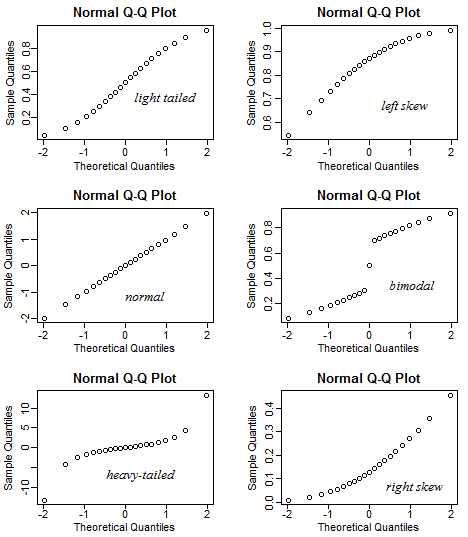
\includegraphics[width=0.6\textwidth]{figures/ch2/qqplot-tutorial}
	\caption{ How information about may be extracted from QQplots. Source: "How to interpret a QQ plot" [Online]. Available: \href{https://stats.stackexchange.com/questions/101274/how-to-interpret-a-qq-plot}{https://stats.stackexchange.com/questions/101274/how-to-interpret-a-qq-plot} [Accessed 09 June 2017]}
	\label{fig:qqplot-tutorial}
\end{figure*}


Another way to analyze scalling characteristics is through QQplots. QQplot is a visual method to compare sample data with a specific stochastic distribution. It orders the sample data values from the smallest to largest, then plots it against the expected value given by the probability distribution function. The data sample values appear along the y-axis and the expected values along the x-axis. The more linear, the more the data is likely to be expressed by this specific stochastic distribution.

Dependent on how the plot behaves, some features of the empirical dataset compared to the theoretical can be observed. In the figure ~\ref{fig:qqplot-tutorial} is presented a summary. 


%%%%%%%%%%%%%%%%%%%%%%%%%%%%%%%%%%%%%%%%%%%%%%%%%%%%%%%%%%%%%%%%%%%%%%%%%%%%%%%%
\subsection{QoS/QoE Related Metrics}

For the point of view of a traffic generation, is interesting that the QoS and QoE metrics present similar values to the ones found in real scenarios. As stated by Magyesi and Szabó\cite{validate-trafficgen}, important QoS/QoE metrics on validation of workload tools are Roundtrip Time values (RTT), average queue waiting time and queue size. Still, on queue size, self-similar traffic consumes router buffers faster than Poisson traffic\cite{multi-player-online-game-self-similarity}.


\section{Conclusions}

In this chapter, we review and discussed some fundamental concepts of our research: network traffic generators, network traffic modeling, and network traffic generators validation. In the section ~\ref{sec:traffic-gen} we surveyed types of traffic generators, and a comparison between its considerable variability of features. It helped us to summarize and have a deep understanding of what is available today for use, and define its gaps. Also, it helped us to see find what tools and frameworks are possible for us to use. In the section ~\ref{sec:modeling-traffic} create a brief overview putting together efforts on network traffic modeling and realistic traffic generation. On modeling, we made a short historical summary of some critical points, and on practical traffic generation, we discussed some reference tools.


%%%%%%%%%%%%%%%%%%%%%%%%%%%%%%%%%%%%%%%%%%%%%%%%%%%%%%%%%%%%%%%%%%%%%%%%%%%%%%%%
%\section{An short overview of some Network emerging scenarios}

%\textcolor{red}{TODO}

%%%%%%%%%%%%%%%%%%%%%%%%%%%%%%%%%%%%%%%%%%%%%%%%%%%%%%%%%%%%%%%%%%%%%%%%%%%%%%%%
%\subsection{SDN: Software Defined Networks}

%\textcolor{red}{TODO}

%%%%%%%%%%%%%%%%%%%%%%%%%%%%%%%%%%%%%%%%%%%%%%%%%%%%%%%%%%%%%%%%%%%%%%%%%%%%%%%%
%\subsection{NFV: Network Function Virtualization}

%\textcolor{red}{TODO}

%For NFV instrumentation and benchmark, there are still few works aiming this gap. \cite{instrumentation-framework-nfv} create a web-based framework for NFV instrumentation in bare-metal and embedded level, but the source code is not provided. \cite{nfv-benchmarking-fault} implement some use cases of NFVIs (Network Function Virtualization Infrastructures) based on fault injection. \cite{nfpa-paper} implement an open-source tool, called NFPA, focusing on benchmarking of Network Functions. 
